\newpage
\section{Systemöversikt}
QuadOpt är uppdelat i flera mindre moduler, som syns i figur \ref{fig:arkitektur}, för att vara mer lätthanterligt och lättare att utveckla.

\begin{itemize}
\item \textbf{solver} - innehåller lösningsalgoritmen samt hjälpfunktioner
\item \textbf{matrixlibrary} - innehåller funktioner och datatyper för matrisaritmetik
\item \textbf{MATLAB-gränssnitt} - gränssnittskod mellan solver och MATLAB
\item \textbf{GUI} - grafiskt gränssnitt
\item \textbf{parser} - tolkar problem- och datafiler och genererar C-kod (solution.c)
\end{itemize}

\noindent Av dessa moduler är solver, matrixlibrary och MATLAB-gränssnittet skrivna i C. GUI samt parser är skrivna i Python 3.
\newline
\newline
Användaren har möjligheten att använda QuadOpt antingen via MATLAB eller via gruppens egna GUI. Om MATLAB används kommer den inskickade datan att konverteras till QuadOpts datastrukturer via en specialfunktion skriven i C som förklaras mer exakt i avsnitt 4.2. Skulle istället GUI:t att användas, så kommer datan att konverteras från QuadOpt-filformatet till en C-fil (solution.c) av en parser. C-filen kompileras tillsammans med QuadOpts kod innehållande alla datastrukturer som behövs, detta beskrivs senare i avsnitt 4.5. Hur själva solvern fungerar och löser problemet beskrivs i avsnitt 4.1. Matrisbiblioteket som solvern använder innehåller de matrisoperationer som behövs, detta beskrivs i avsnitt 4.3.

\begin{figure}[H]
\centering
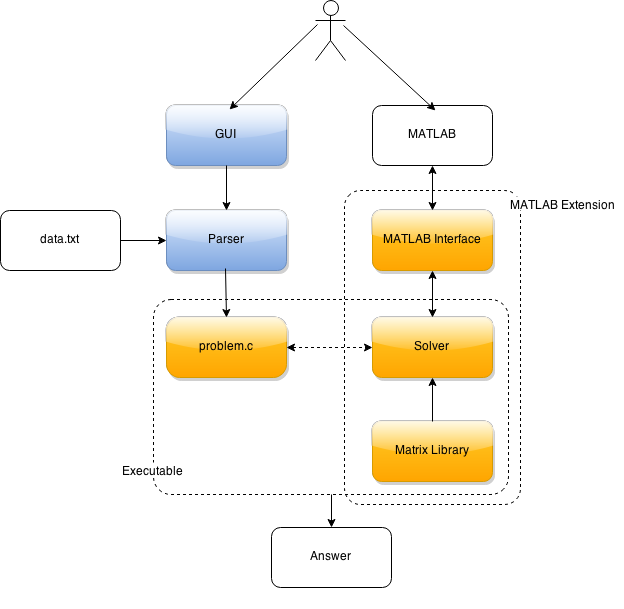
\includegraphics[scale=0.5]{bilder/arkitektur.png}
\caption{Arkitektur av systemet.}
\label{fig:arkitektur}
\end{figure}
